\documentclass[type=dr, dr=rernat, acm$^3$entcolor=tud7b,colorbacktitle, bigchapter, openright, twoside, 12pt ]{tudthesis}
%\documentclass[11pt,twoside,a4paper]{article}
\usepackage[english]{babel} 
\usepackage[utf8]{inputenc}
\usepackage{graphicx}
\usepackage{pstricks}
\usepackage{psfrag}
\usepackage{enumerate}
\usepackage{float}
\usepackage{epsfig}
\usepackage{geometry}
\usepackage{subfigure}
\usepackage{rotating}
\usepackage{minitoc}
\usepackage{multirow}
%\usepackage{appendix}

%%%% 1 1/2 facher Zeilenabstand:	
\usepackage{setspace}
\onehalfspacing




\begin{document}
\chapter{Comparison of Photons versus Carbon Ions in Single Fraction Therapy of Lung Cancer}
\label{PatStudy}


\section{Introduction}

Lung cancer is one of the leading medical problems worldwide with approximately 1.4 million deaths per year [1]. Surgery is usually the first choice in treating localized non-small cell lung cancer (NSCLC). However, in recent years stereotactic body-radiation therapy with photons (SBRT) showed very promising results, with high local control-rates of NSCLC  \cite{Baumann2009, Fakiris2009, Grutters2010, Ricardi2010, Timmerman2010, Greco2011}.

Scanned particle therapy can produce sharp dose gradients with a finite range of the beam and can thus provide higher healthy tissue sparing. This reduces both side effects as well as the risk of secondary cancer \cite{Newhauser2011}. Treatment of lung tumors with particles is still challenging due to interplay and radiological path length changes [9]. The latter can be substantial when dense tissue (e.g. the solid tumor mass) is replaced with low-density tissue (lung) due to motion.

Grutters et al. have performed a meta-analysis on comparison between photon, proton and carbon ions in treating NSCLC \cite{Grutters2010}. They found similar 5-year survival rates for SBRT, protons and carbon-ions (around 40\%). However, the number of patients treated with particle therapy was low and they advise caution when interpreting the data. Also different fractionation schemes were used in the comparison. A more recent review was published by  Kamada et al. [10] where they reported a high 3-year survival rate for single-fraction carbon-ions (76.9\%), with no late treatment-related adverse effects. In comparison, SBRT had 55.8\% 3-year survival rate, with 10 – 27\% of patients exhibiting grade 3 treatment-related adverse effects. [6]. It is important to note that all of these studies used passive beam scattering, avoiding the problem of interplay between organ motion and scanning beam motion. On the other hand, active beam scanning can provide even better dose shaping which becomes essential in high dose single fractionation regimes. The effects of motion and motion mitigation techniques on scanned carbon ion dose distribution therefore need to be considered in a fair comparison of photons and carbon ions. 

To evaluate potential advantages of active scanning with carbon ions (PT), an in silico comparison of simulated PT plans to SBRT plans actually delivered was conducted. Target coverage and a wide range of OAR doses were assessed both with and without simulated motion on time-resolved computed tomographies (4D-CTs).



\section{Materials and methods}

\subsection{Patient data}

The study included 19 patients with in total 26 lesions that were actually treated with SBRT at the Champalimaud Centre for the Unknown, Lisbon (Portugal). The lesion size was 2.9 cm$^3$ (median, 25-75\% 1.4 – 9.7) and peak-to-peak motion was 3.1 mm (1.6 – 5.6). Three patients had two targets, one had five and the rest one. 13 lesions were right-sided, 12 were left-sided and one was located in right cardiophrenic space. An overview of tumor characteristics can be found in Table~\ref{tab:paddata}.
Two CTs were available for all patients. A planning CT was used for OAR delineation and SBRT planning. Target motion was estimated on a 4D-CT, consisting of 10 phases (0\% - 90\%). Clinical target volumes (CTV) were delineated using a registered positron emission tomography (PET) scan.
The planning objectives were that 99\% of planning target volume (PTV) must receive at least 24 Gy (D_{99}\% $\geq$ 24 Gy) in a single fraction, while all OAR constraints as defined in the AAPM task group 101 report on stereotactic radiotherapy had to be respected \cite{Benedict2010}.

\begin{table}[H]
  \centering
%   \footnotesize
  \caption{Lesion characteristics, with lesion locations, stages, peak-to-peak motions and volumes of corresponding CTV, PTV$_{SBRT}$ and PTV$_{PT}$. Abberevations for lesion location are: 
  RSL, right superior lung; IRL, inferior right lung; LSL, left superior lung; ILL, inferior left lung; RCS, right cardiophrenic space.}
  \begin{tabular}{|c|c|c|c|c|c|c|}
    \hline\hline
     & & & & \multicolumn{3}{|c|}{Volume (cm$^3$)} \\ \cline{5-7}
    \multirow{2}{*}{Number} & \multirow{2}{*}{Location} & \multirow{2}{*}{Stage} &
    Peak-to-peak & \multirow{2}{*}{CTV} & \multirow{2}{*}{PTV$_{SBRT}$} & \multirow{2}{*}{PTV$_{PT}$}\\
     &  & & motion [mm] & & & \\
    \hline
    1 & LSL & IIa & 4.8 & 35.9 & 100 & 179 \\
    2 & LSL & Ia & 3.1 & 1.6 & 7.7 & 40.6 \\
    3 & IRL & IV & 12 & 2.3 & 11.6 & 32 \\
    4 & RSL & Ia & 0.5 & 6.9 & 25.2 & 38 \\
    5 & ILL & IV & 4.4 & 2.5 & 15 & 20.5 \\
    6 & ILL & IV & 7.5 & 1.4 & 7.7 & 26.5 \\
    7 & RSL & IV & 3.9 & 16 & 40 & 72.5 \\
    8 & ILL & IV & 0.6 & 139 & 261 & 255 \\
    9 & LSL & IV & 2 & 9.2 & 35 & 46.5 \\
    10 & IRL & IV & 3.4 & 10.2 & 38 & 45.5 \\
    11 & ILL & IV & 2.8 & 14.4 & 46.4 & 57.2 \\
    12 & ILL & IV & 5.8 & 3.8 & 17.4 & 23.4 \\
    13 & RSL & IV & 0.8 & 4.3 & 17.7 & 26.3 \\
    14 & LSL & IV & 3.4 & 2.7 & 14.5 & 23.1 \\
    15 & RSL & IV & 2.1 & 3.1 & 15.4 & 33.5 \\
    16 & LSL & IV & 0.5 & 0.5 & 5.4 & 6.7 \\
    17 & ILL & IV & 7.8 & 0.8 & 6.1 & 23.5 \\
    18 & LSL & IV & 0.1 & 1.7 & 15 & 23.5 \\
    19 & IRL & IIIb & 11.4 & 27 & 137 & 118.5 \\
    20 & RSL & Ia & 2.2 & 1.7 & 10 & 23.4 \\
    21 & RSL & IV & 0.2 & 0.9 & 3.2 & 14.9 \\
    22 & RSL & IV & 2.2 & 3.9 & 22.1 & 27.5 \\
    23 & LSL & IV & 3.1 & 9.8 & 28 & 51 \\
    24 & RSL & IV & 8.1 & 0.6 & 3.3 & 4.1 \\
    25 & LSL & IV & 1.4 & 0.8 & 5.9 & 10 \\
    26 & RCS & IV & 11.8 & 0.4 & 6.6 & 8.6 \\

    \hline\hline
  \end{tabular}
  \label{tab:patdata}
\end{table}

\subsection{Planning target volume definition}

To account for range changes relevant for particles only, different PTV definitions were used for SBRT and PT, as shown in Fig.~\ref{Fig:PTV_def}. Within this chapter they will be named PTV$_{SBRT}$ and PTV$_{PT}$ for SBRT and PT, respectively.
In SBRT, the responsible clinician determined the maximum breathing motion of the CTV from the 4D-CT, hence creating an ITV. This ITV plus an additional 3 mm for setup uncertainty yielded the PTV$_{SBRT}$.

PTV$_{PT}$ was constructed following principles from Graeff et al \cite{Graeff2012}. Each beam has a unique PTV$_{PT}$. For setup uncertainty margins of 3 mm laterally and 1 mm in beam’s eyes view (BEV) were used on the CTV. Afterwards a water-equivalent path length ITV (WEPL-ITV) was build, using transformation maps from the B-Spline deformable registration of the 4D-CT data \cite{Shackleford2010}. Additional 2 mm + 2\% proximal and distal margins were added in BEV to account for uncertainty from Hounsfield units to water equivalent path length conversion.
If the target overlapped with an OAR (e.g. small airways) then OAR plus a margin of 2-5 mm was subtracted from PTV$_{SBRT}$ or PTV$_{PT}$.


\begin{figure}[H]
\begin{center}
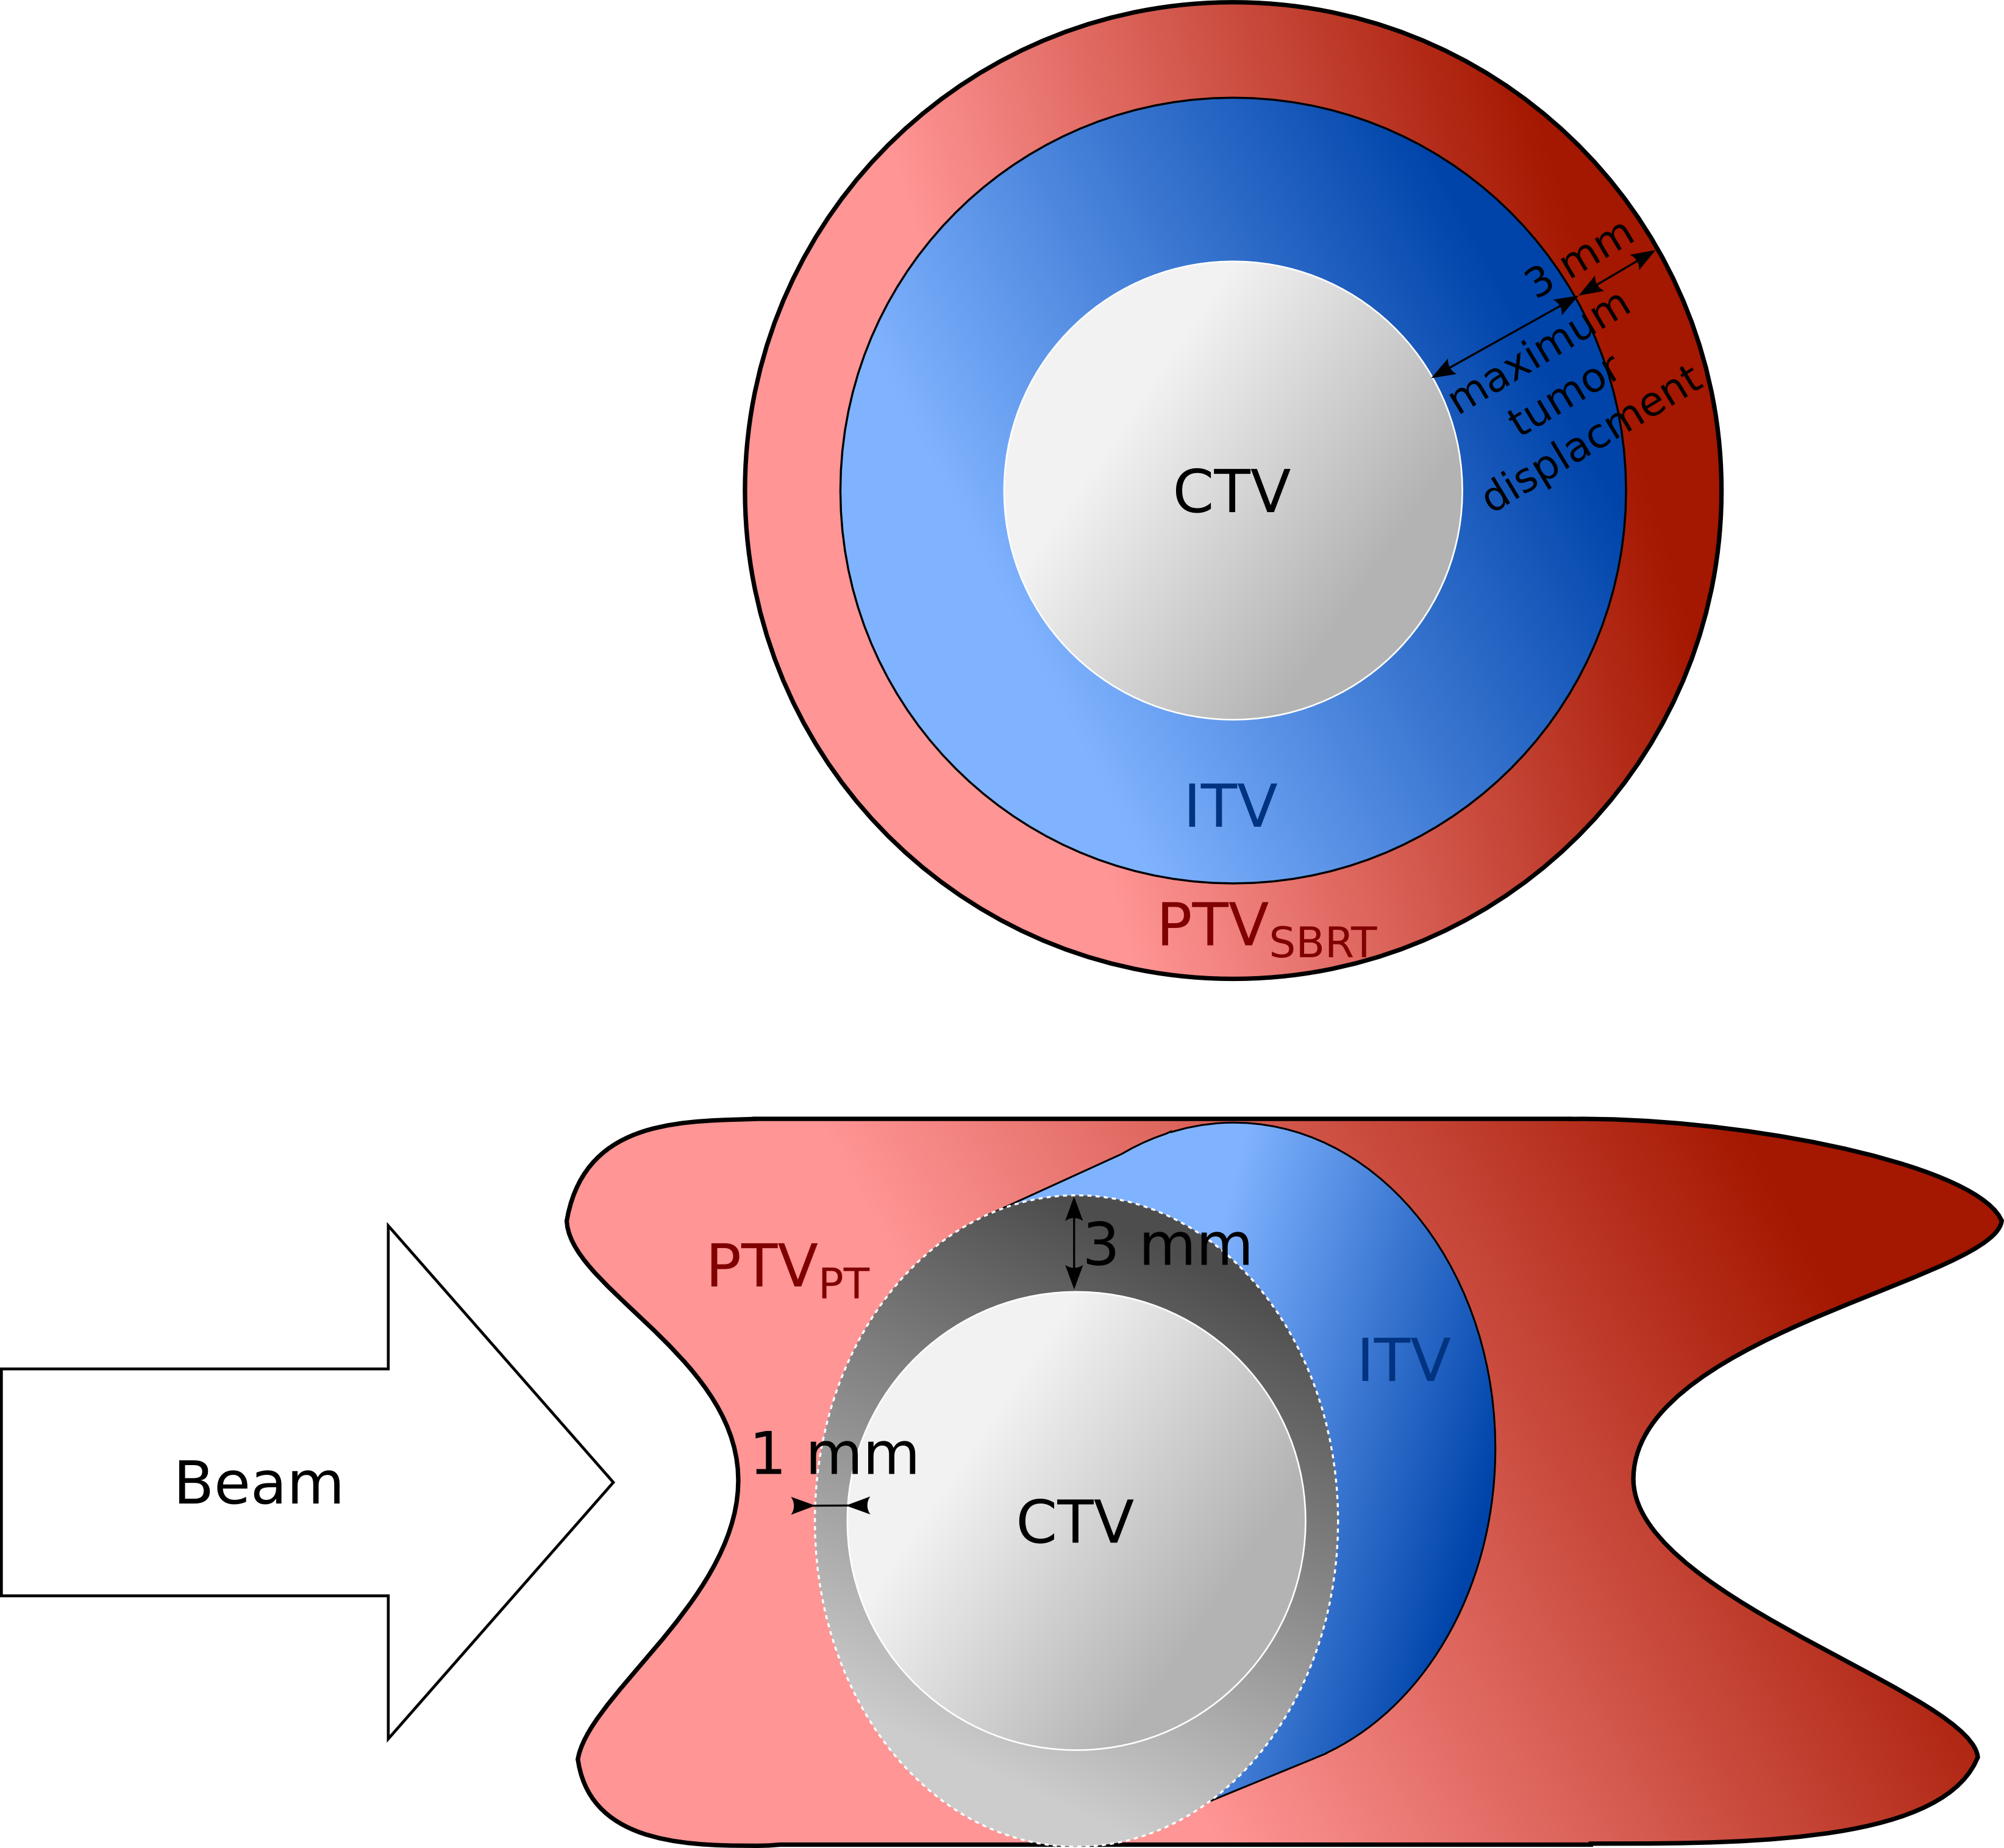
\includegraphics[width=0.9\textwidth]{./Images/Figure1.png}
\caption{Different PTV definitions for SDRT (PTV$_{SBRT}$) and CiT (PTV$_{PT}$). For PTV$_{SBRT}$ isotropic margins of 3 mm plus maximum tumor displacement due to 
breathing were used on the CTV; For PTV$_{PT}$ margins of 3 mm laterally and 1 mm in beam’s eye view were used and then range-ITV was constructed with
2 mm + 2\% range margins added for PTV$_{PT}$ in end-inhale phase.}
\label{Fig:PTV_def}
\end{center}
\end{figure}


\subsection{SDRT treatment planning}
\label{SBRTTP}

The clinical plans were calculated with the Eclipse v10 planning system (Varian Medical Systems, Palo Alto, USA) using the AAA beam model. They were all VMAT plans generally consisting of 4 overlapping partial arcs, 2 in clockwise and 2 anticlockwise direction, with a gantry range of typically 200°. For tumor sizes > 2.5 cm a calculation grid of 2.5 mm was used, otherwise this was 1 mm. During optimization, a first iteration included the PTV$_{SBRT}$ only, after which the OARs were added. In order to lower OAR dose and improve the PTV$_{SBRT}$ homogeneity, we created an artificial shell of 2 cm around the PTV$_{SBRT}$ and minimized the dose there as well. During optimization the fast Multi Resolution Dose Calculation (MRDC) model was used, with one intermediate step using the slower but more accurate AAA model to get an adequate PTV$_{SBRT}$ coverage after optimization.


\subsection{CiT treatment planning}
\label{CiTTP}

For PT, state of the art 4D treatment planning software TRiP98 was used \cite{Richter2013}. A single field uniform dose plan (SFUD) was optimized on the PTV$_{PT}$ in the end-inhale reference phase of the 4D-CT. Most targets ($n=20$) were planned with two fields. For the remaining targets, one ($n=1$), three ($n=3$) or four ($n=2$) fields were used due to proximity of OARs. A regular grid of beam spots with a spacing of 2 mm, a beam spot full width at half maximum (FWHM) size of approximately 6 mm and a 3 mm ripple filter were used. To compensate for short particle ranges in lung tissue, a bolus of 80 mm water-equivalent thickness was added.

The relative biological effectiveness (RBE) following the local effect model (LEM) IV [15]. For a conservative estimation, an alpha-beta ratio of 6 Gy and 2 Gy were used for target and OARs, respectively. This led to an RBE of approximately 1.1 in target tissue and approximately 1.1 to 3 in OARs.
Dose was calculated on end-inhale (3D-Dose$_{0\%}$) and end-exhale (3D-Dose$_{50\%}$) phases. 4D dose delivery was simulated as described by Richter et al [16]. Two different breathing periods (3.6 and 5 s) and two different starting phases (0° and 90°) were used. Simulations without motion compensation (4D-Dose$_{interplay}$) and with slice-by-slice raster rescanning were performed (4D-Dose$_{rescan}$). Five rescans were used for the majority of targets (n=24), whereas 20 rescans were used for targets where the interplay effects were too big to achieve a satisfactory target coverage ($n=2$; lesions 3 and 18 in Table~\ref{tab:patdata}). 


%\begin{figure}[H]
%\begin{center}
%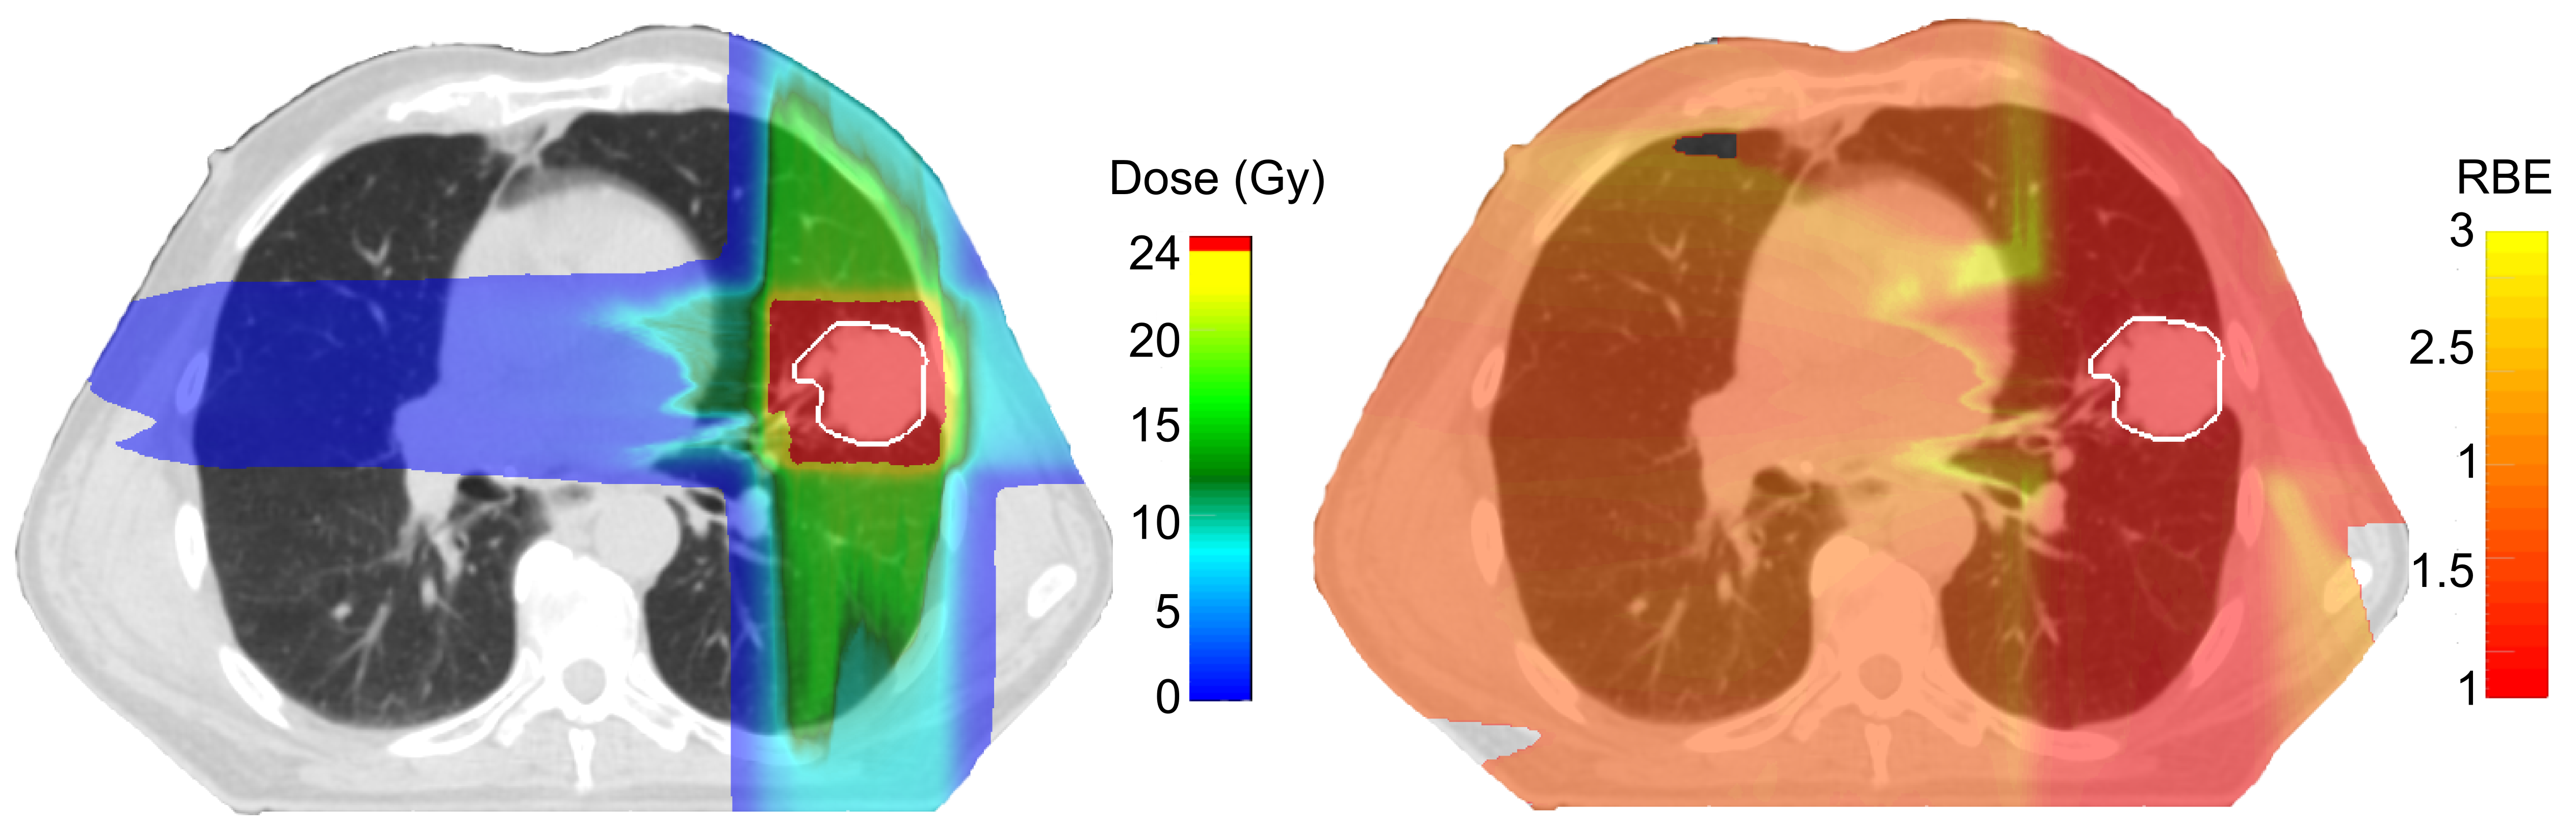
\includegraphics[width=0.9\textwidth]{./Images/RBE.png}
%\caption{RBE distribution in a patient (a) depends on a actual dose profile (b).}
%\label{Fig:RBE}
%\end{center}
%\end{figure}

\subsection{Dose metrics and analysis}

For comparison between SBRT and PT the following dose metrics were used – for the target the minimum dose in 99\% of the volume (D$_{99\%}$), which should be higher than 24 Gy; for OARs, the maximum point dose ($D_{Max}$) and the mean dose ($D_{Mean}$). Additionally, the volume receiving 20\% of the planned dose ($V_{20\%}$) was used to assess differences in lung doses. In all cases, absorbed dose in Gy for SBRT was compared to biologically-equivalent dose in Gy(RBE) for PT.

Paired t-tests were performed to compare the dose metrics and for post-hoc exploratory analysis between groups a two-sided t-test with Welch correction for different variances was carried out. A p-value < 0.05 was considered significant. Dose differences are always reported such that higher dose levels for SBRT result in positive values.



\section{Results}

Examples of two SBRT and 4D-Dose$_{rescan}$ PT treatment plans are shown in Fig.~\ref{Fig:TreatmentPlans}. Patient 9 has two lesions in close proximity to the spinal cord. Patient 2 has a small lesion (1.6 cm$^{3}$) in the superior position of the left lung. D$_{99\%}$ is 100\% for SBRT and PT in all CTVs for Patient A and B; average OAR difference between SBRT and PT in $D_{Max}$ is 5.1 Gy and 1.4 Gy and in mean dose 1.4 Gy and 0.7 Gy, respectively for patient A and B.


\begin{figure}[H]
\begin{center}
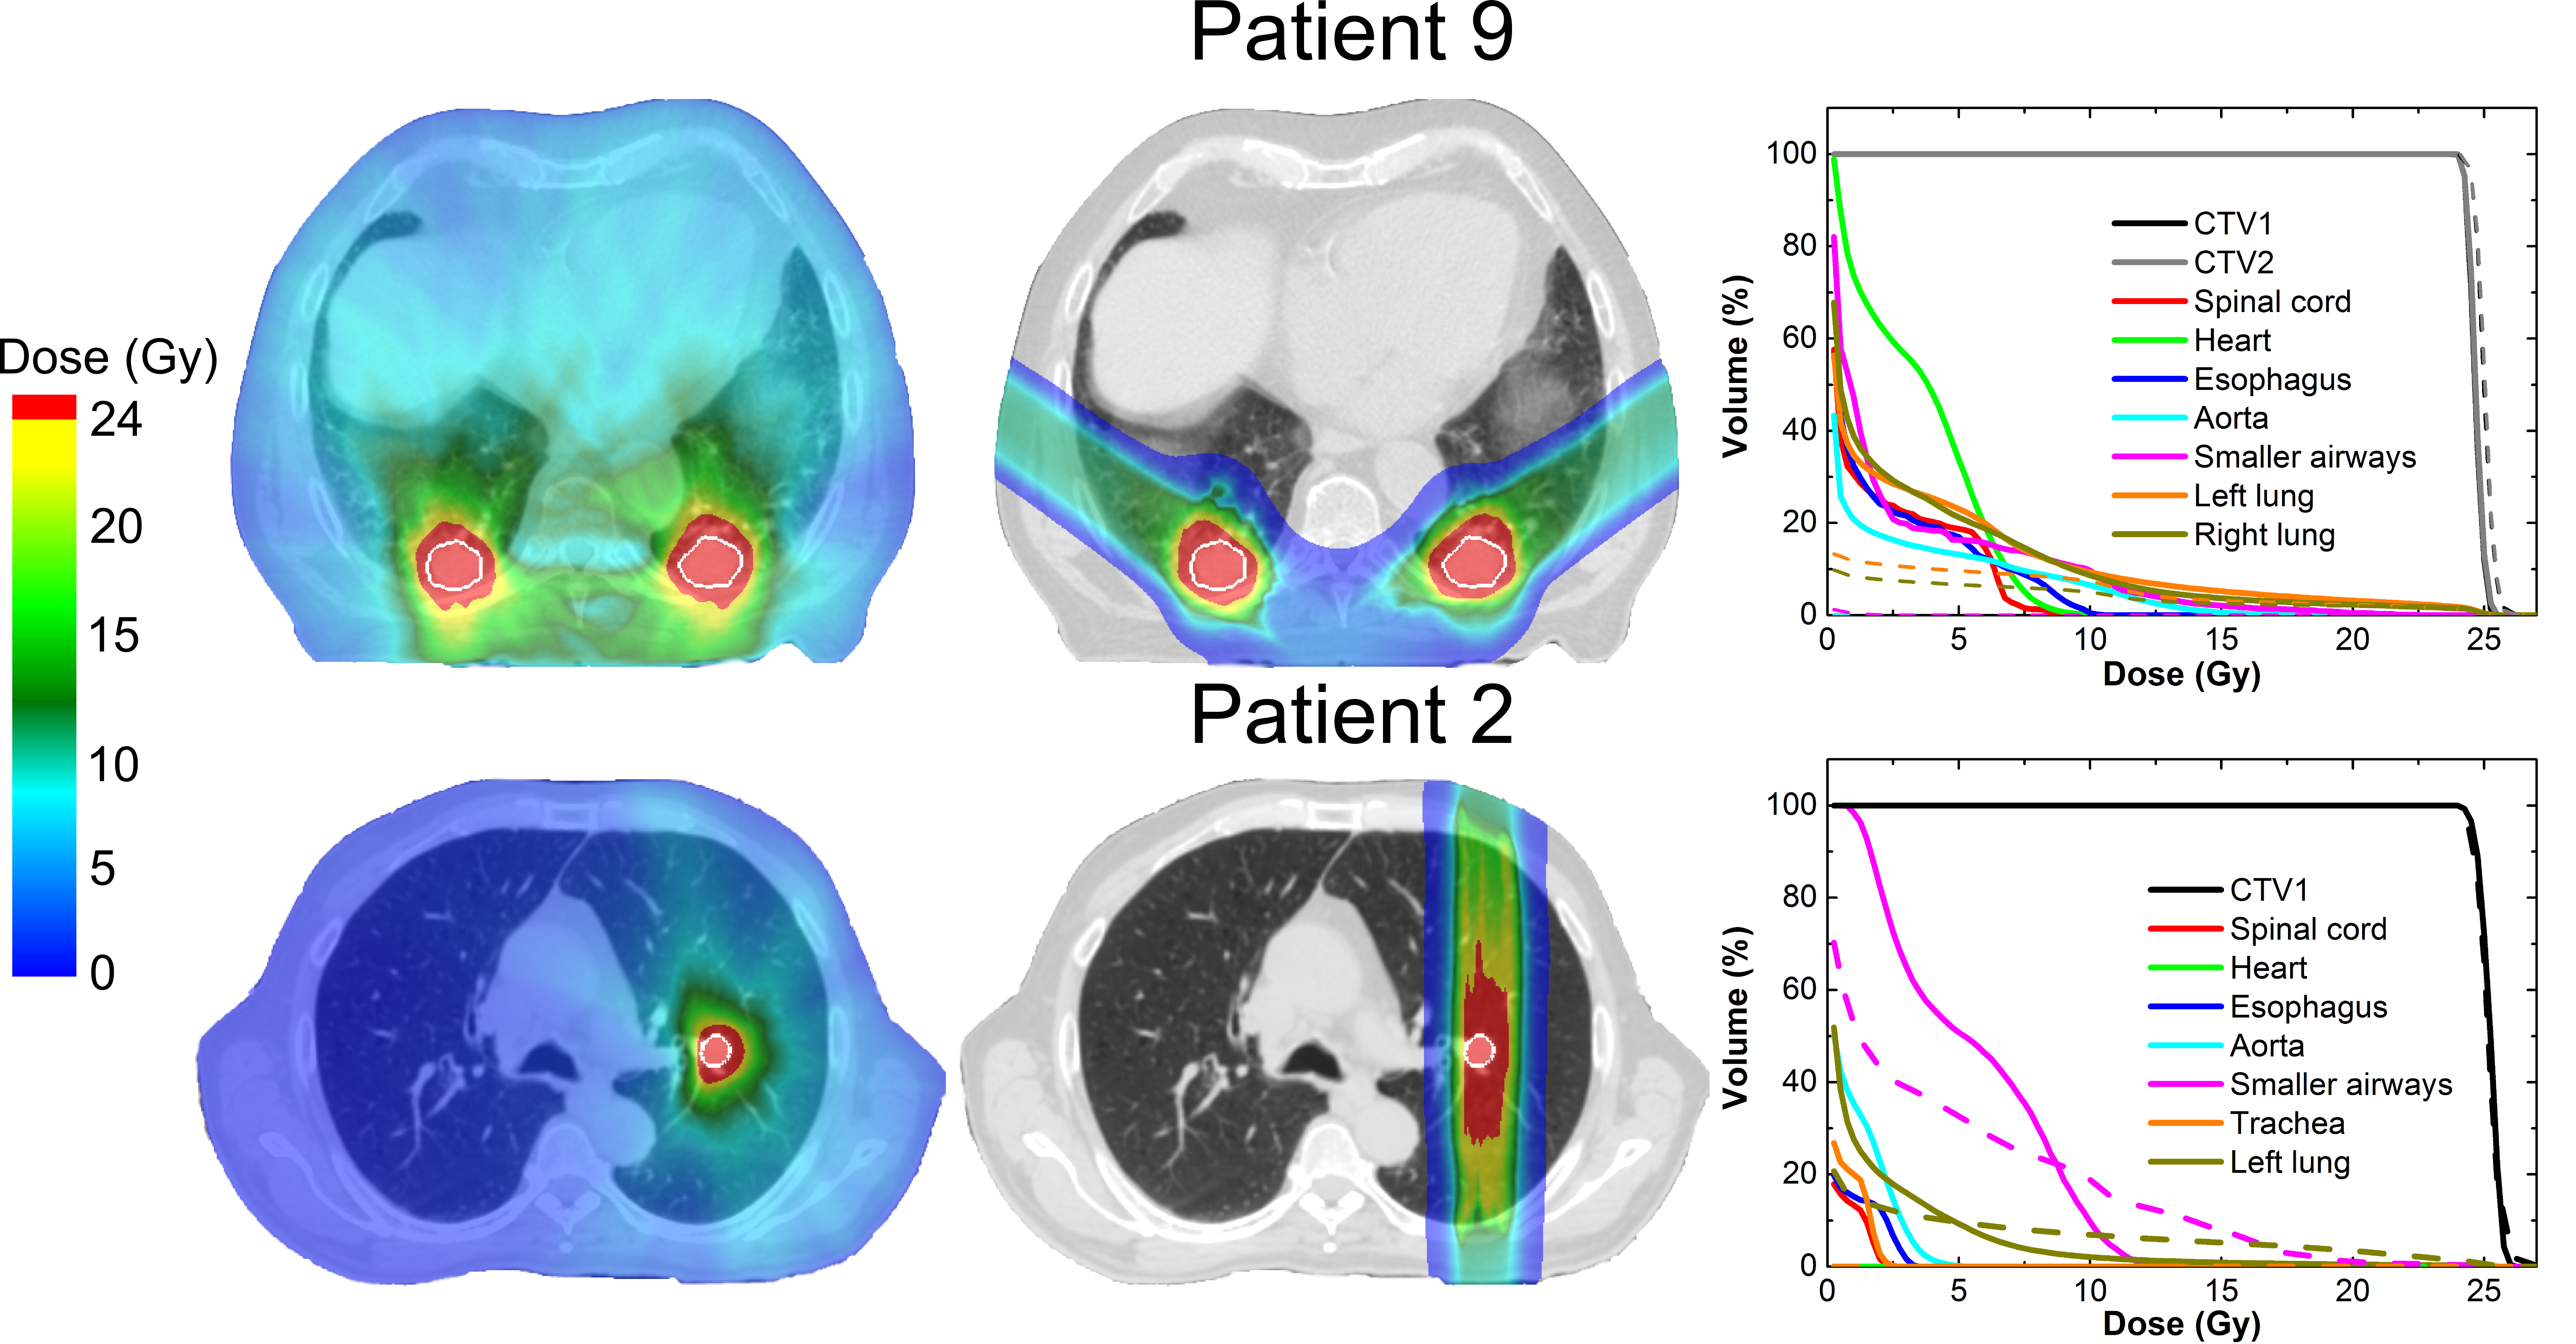
\includegraphics[width=0.9\textwidth]{./Images/Figure2.png}
\caption{Treatment plans for SBRT (left), PT (middle) and dose volume histogram (right) for SBRT (solid lines) and PT (dashed lines) for two patients. PT curves for OARs without any dose are not shown. Patient 9 (top row) might be better suited for PT and patient 2 (lower row) for SBRT. Patient 2 has a small lesion (1.6 cm$^{3}$) in a central lung region, resulting in large PTVPT - up to 32 cm$^{3}$, compared to PTVSBRT 7.7 cm$^{3}$. The CTV contour is outlined in white.}
\label{Fig:TreatmentPlans}
\end{center}
\end{figure}

\subsection{Target Coverage}

Difference in PTV definition resulted in 1.5 (1.3 – 2.1) times bigger PTV$_{PT}$ than PTV$_{SBRT}$. All SBRT plans were clinically acceptable, though in one case the D$_{99\%}$ was reduced to 16.8 Gy due to proximity of an OAR. 3D-Dose$_{0\%}$ and 3D-Dose$_{50\%}$plans provided sufficient target coverage in all patients. For 4D-Dose$_{interplay}$ and 4D-Dose$_{rescan}$ there was 63\% and 2\% cases of insufficient target coverage, respectively, across all targets and different breathing patterns. Details are shown in Fig.~\ref{Fig:InterplayDiff}. For the patient with reduced dose in SBRT, PT could increase the D$_{99\%}$ from 16.8 Gy in SBRT to 20.3 Gy while adhering to OAR constraints. 


\begin{figure}[H]
\begin{center}
\includegraphics[width=0.9\textwidth]{./Images/Figure3.png}
\caption{CTV D$_{99\%}$ for SBRT and different PT calculations. Four different breathing patterns are included for all targets in 4D-interplay and 4D-rescan. The dashed line shows the lower limit for clinical acceptance. One patient was an exception where lower target dose was accepted due to the proximity of a critical structure.  }
\label{Fig:InterplayDiff}
\end{center}
\end{figure}

\subsection{Dose in OARs}


There was no significant difference in dose to OAR between the different PT dose calculations. The $D_{Max}$ and $D_{Mean}$ for SBRT and 4D-Dose$_{rescan}$ for OARs heart, spinal cord, smaller airway esophagus, trachea, aorta, ipsi- and contralateral lung are presented in Table~\ref{tab:results}.There was a significant difference in both $D_{Max}$ and $D_{Mean}$ for all OARs between SBRT and PT, with PT delivering less dose to OARs. Significant difference was also observed for $V_{20\%}$ for ipsilateral lung, which was 15.3\% (9.6 – 23.5) and 10.3\% (7.9 – 13.7) for SBRT and PT, respectively. The $V_{20\%}$ for contralateral lung was zero for almost all patients in SBRT and PT. The overall OAR difference for patients between SBRT and PT was significant, 2.8 Gy (1.6– 3.7)  for $D_{Max}$ and 0.7 Gy (0.3– 1.6) for $D_{Mean}$. 



\begin{table}[H]
  \centering
%   \footnotesize
  \caption{Dose metrics for OARs. First value at each organ is from SDRT and the second from 4D-rescan. All values are shown as median and 25-75\% in brackets.}
  \begin{tabular}{l|c|c|c|c|}
    \cline{2-5}
     & \multicolumn{2}{|c|}{$D_{Max}$ (Gy)} & \multicolumn{2}{|c|}{$D_{Mean}$ (Gy)} \\
     \hline
    \multicolumn{1}{|l|}{OAR} & Photon & Carbon & Photon & Carbon	\\
    \hline
\multicolumn{1}{|l|}{Heart} & 6.0 (0.3 – 11.6) & 0 (0 – 8.8)	& 1.3 (0.1 – 2.2) & 	0 (0 – 0.5) \\
\multicolumn{1}{|l|}{Spinal Cord} &	5.5 (3.3 – 8.5)	& 0 (0 – 0.5) &	0.7 (0.3 – 1.2) &	0 (0 – 0) \\
\multicolumn{1}{|l|}{Smaller Airways} & 13.0 (9.8 – 17.1) &	10.3 (3.3 – 19.1) &	2.8 (1.5 – 5.8) &	0.5 (0 – 2.6) \\
\multicolumn{1}{|l|}{Esophagus} & 5.8 (3.9 – 8.4) &	0 (0 – 0.3) &	1.1 (0.6 – 1.5) &	0 (0 – 0)\\
\multicolumn{1}{|l|}{Trachea} &3.9 (1.8 – 5.4) &	0 (0 – 0) &	1 (0.3 – 1.3) &	0 (0 – 0)\\
\multicolumn{1}{|l|}{Aorta} & 8.0 (5.1 – 21.9) &	3.9 (0 – 18.1) &	1.4 (0.7 – 1.6) &	0.1 (0 – 0.4)\\
\multicolumn{1}{|l|}{Ipsilateral Lung} & 26.3 (26.0 – 26.5) &	26.3 (25.8 – 26.5) &	1.9 (1.5 – 3.0) &	1.9 (1.4 – 2.5)\\
\multicolumn{1}{|l|}{Contralateral Lung} & 5.0 (3.5 – 9.6) &	0 (0 – 0.9) &	0.4 (0.2 – 0.6) &	0 (0 – 0) \\
    \hline\hline
  \end{tabular}
  \label{tab:results}
\end{table}




\subsection{Dependence on CTV Size}

Significant differences were observed between patients with a single CTV smaller ($n=8$) or larger ($n=7$) than 2.5 cm$^{3}$ for $D_{Max}$ and $D_{Mean}$, see Fig.~\ref{Fig:OAR_boxplots}. For patients with a smaller CTV, the dosimetric advantage over SBRT was on average 0.9 Gy and 0.5 Gy lower for $D_{Max}$ and $D_{Mean}$, respectively. This was associated with PTV$_{PT}$ definition - the average volume ratio between PTV$_{PT}$ and PTV$_{SBRT}$ was 2.9 (1.6 – 4.0) and 1.5 (1.3 – 1.8), for patients with CTV < 2.5 cm$^{3}$ and CTV > 2.5 cm$^{3}$, respectively.

The 4 patients with multiple lesions were excluded from this comparison. The $D_{Max}$ and $D_{Mean}$ difference were on average higher in these patients, but the number of patients was too low for statistical analysis. 


\begin{figure}[H]
\begin{center}
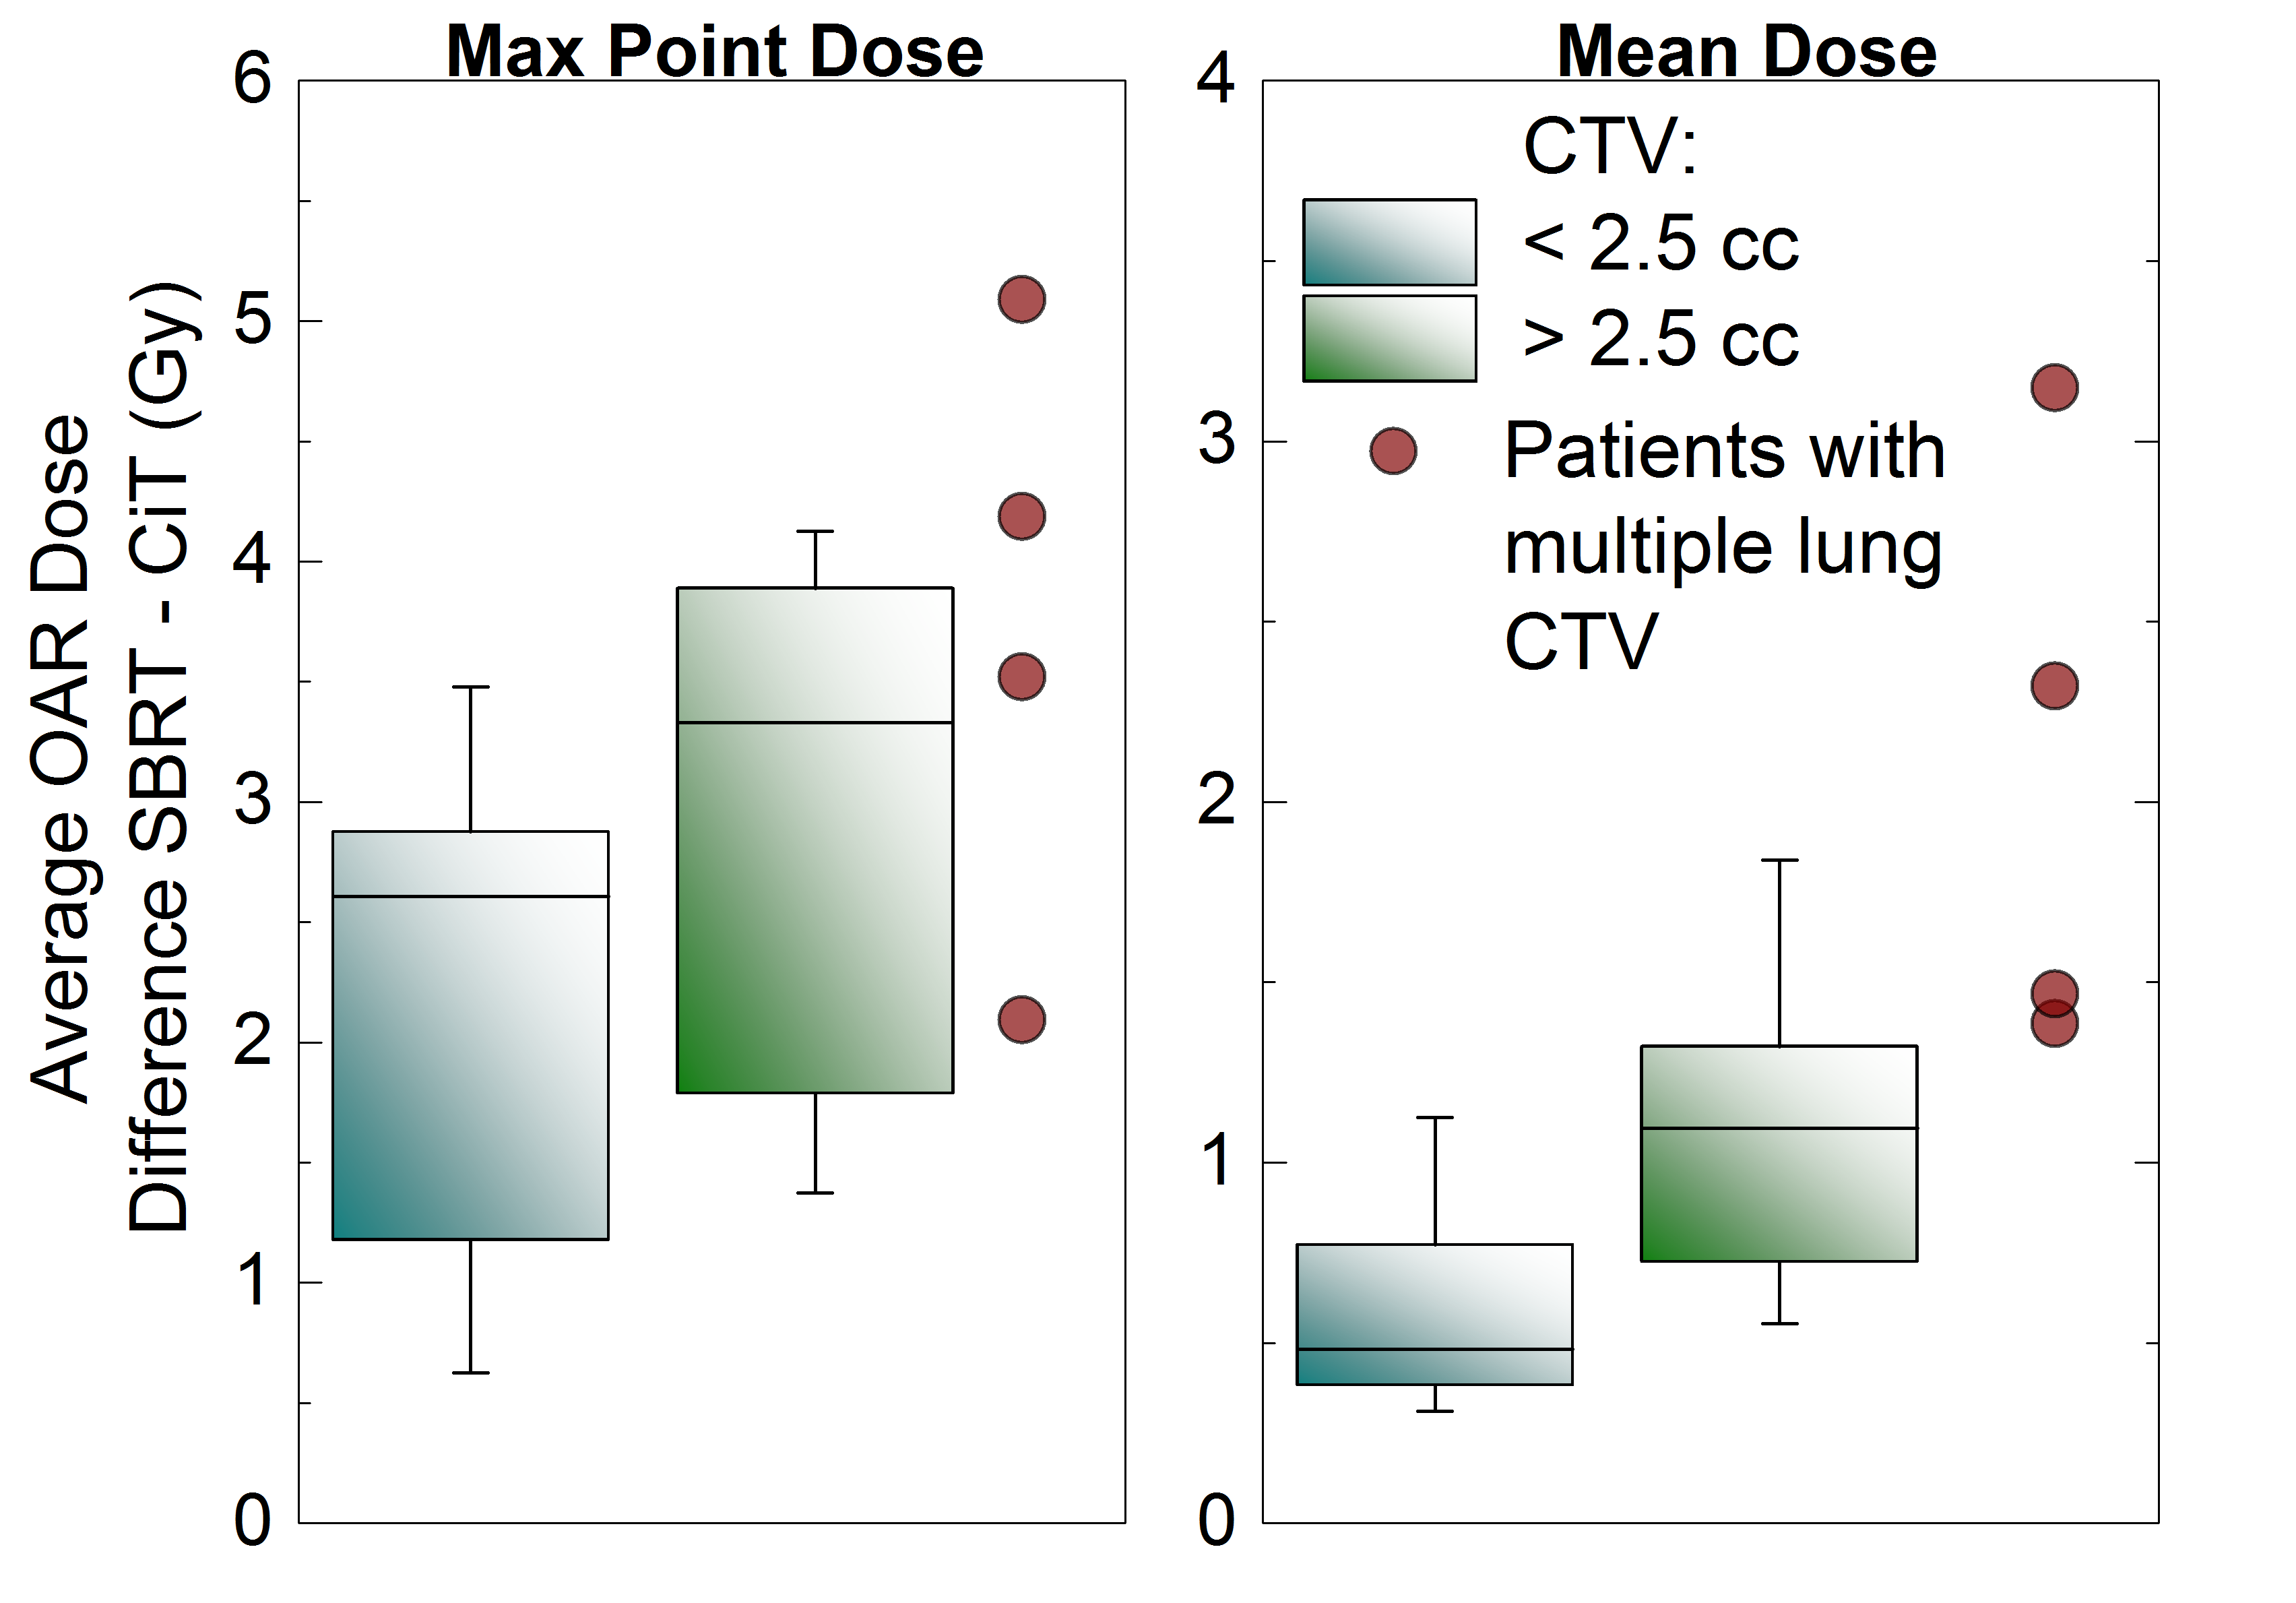
\includegraphics[width=0.9\textwidth]{./Images/Figure4.png}
\caption{Box plots of average OARs max point dose ($D_{Max}$) and mean dose difference between SBRT and PT for patients with single CTV smaller ($n = 9$) or bigger ($n = 6$) than 2.5 cm$^{3}$. Boxes represent 25\% - 75\%, outliers are shown as whiskers and median is shown with solid lines. Values for patients with multiple lesions are shown with circle symbols.}
\label{Fig:OAR_boxplots}
\end{center}
\end{figure}


\section{Discussion}

This is the first in silico trial directly comparing clinically valid SBRT plans to scanned carbon ion plans using state of the art 4D dose calculation and motion mitigation methods for NSCLC patients. Our study found that PT deposited less dose to OARs compared to SBRT. Therefore PT might be considered as an alternative treatment option to SBRT. The finite range of the beam permits a small number of fields and thus a narrow entry channel, so that critical OARs such as spinal cord, heart, esophagus, and the contralateral lung could be effectively spared using PT, with typically low or even zero dose. PT could be thus highly beneficial to patients with impaired contralateral lung function, because PT deposited no dose in the contralateral lung in 12 patients, while SBRT irradiated the contralateral lung in all patients. Being an intensity-modulated arc therapy, SBRT had an advantage in some patients where the smaller airways were in a close proximity to CTV; SBRT could shape the dose distribution to reduce dose to the smaller airways, compensating PT’s advantageous physical dose characteristics.

Further increase in OAR sparing could be achieved by using intensity modulated particle therapy (IMPT) instead of SFUD. While IMPT could lead to less dose in the OARs, it would make the plans less robust against setup errors due to additional dose gradients between the fields. These gradients can be controlled by employing robust optimization to account for range, motion and setup uncertainties, which we will implement in a future 4D treatment planning study \cite{Chen2012}[17,18].



\subsection{Range Margins and Motion Mitigation}

Since conventional geometric margins are not suitable for PT \cite{Park2012}, margins based on range changes were used. Another trial comparing photon to proton therapy in NSCLC patients also used different PTV definitions to incorporate range changes  \cite{Roelofs2012}. As shown in our study, inclusion of range changes leads to increase in PTV$_{PT}$, up to 4.7 times compared to PTV$_{SBRT}$. Furthermore, the difference between PTVs is bigger for smaller tumor sizes. Patients with bigger tumor volumes (CTV > 2.5 cm$^{3}$) are therefore better suited for treatment with PT. 

Our results confirm previously published results that interplay can lead to a dose degradation in treating moving targets with active scanned beam \cite{Bert2008}. Figure 3 shows the importance of using 4D dose calculation and motion mitigation techniques in treating moving targets with particles. Even small motion amplitude can lead to underdosage in CTV without proper motion mitigation. Considering the average over the 4 simulated motion patterns, 15 patients showed a D$_{99\%}$ < 24 Gy under interplay conditions, as opposed to none when using rescanning (excluding the one patient with reduced target dose). Rescanning proved to be a strong mitigation technique, with robust results across all targets and different breathing patterns.

Recent studies suggest that some patients require phase-controlled layer or volumetric rescanning for sufficiently robust target coverage \cite{Mori2013,Takahashi2014}. The advantage of simple slice-by-slice rescanning is that no motion monitoring or assumptions on the breathing frequency are necessary [9], but the higher required number of rescans might increase treatment times due to reduced beam intensities. Another possibility is to combine rescanning with gating, which was already sucm$^{3}$essfully implemented in clinic [24].




\subsection{RBE and Proton Therapy}

Carbon ions exhibit a radiobiological advantage, especially in the Bragg peak region. However, for high doses as used here the effect of RBE is not well documented and is subject to ongoing research \cite{Friedrich2014}. For these high doses RBE for carbon ions should approach a value between 1 and 2 \cite{Carabe2007}, which is in agreement with values in our study ( ~ 1.1).

Coincidently, RBE values in the target at high doses are similar to those used clinically in proton therapy. Carbon-ions show considerably lower lateral scattering though, which should result in even better OAR sparing than protons. Our results are in agreement with several in silico studies comparing SBRT and proton therapy for NSCLC \cite{Roelofs2012, Kadoya2010, Register2010}. Furthermore, a study made by Kadoya reached the same conclusion as our study, that patients with larger CTV and/or multiple CTVs would  receive less dose from proton therapy \cite{Kadoya2010}. A recent phase II trial for patients with multiple sites of extracranial disease showed good results for photons \cite{Iyengar2014}, however, based on the findings of Kadoya et al and our study, proton and/or carbon-ion therapy might result in even better outcome. 



\subsection{Study limitations}


The 4D dose calculations were based on a regular breathing pattern, which typically varies during patient treatment and/or between 4D-CT acquisition and actual treatment \cite{Verma2010, Malinowski2011}. A possible solution was proposed by Boye et al. to get motion information from 4D magnetic resonance imaging (4DMRI) and use it in 4D dose calculations \cite{Boye2013}.

Furthermore, SBRT treatment plans were done on a static case in contrast to a 4D dose calculation done for PT. This should not influence the results of our study, since motion has a smaller impact on photon dose distributions \cite{Zou2014}, whereas it is imperative in PT dose calculations \cite{Bert2011}. 

There were also differences in treatment planning. PT plans were done by a single person in a research setting, whereas SBRT plans were made by different people under clinical conditions with the requirement to finish the plans on time. 

Slight changes also existed between the planning CT, used for SBRT treatment plans and 4D-CT used for PT treatment plans, even though 4D-CT was usually acquired right after the planning CT. The propagation of contours from the planning CT to the 4D-CT and also for the 4D dose calculation rely on deformable image registration (DIR), where even small changes can effect 4D dose distribution \cite{Kashani2008}. Results from DIR were therefore thoroughly checked with different approaches, such as inspection of the warped image, evaluation of the Jacobian values and the inverse consistency of the vector field. However, the transformation of the dose with DIR is a debated topic and might jeopardize the simulated results, especially with respect to the 4D target coverage. On the other hand, dose differences in OARs were large and should be robust against vector field errors in the order a few mm. Nevertheless, further studies are warranted, possibly using advanced moving phantoms for an experimental validation \cite{Perrin2014} and finally also clinical trials. First patients are being treated in thoracic and abdominal regions with an active beam scanning at the National Institute for Radiological Sciences (NIRS) in Japan [36].



\subsection{Application}

Scanned carbon ion therapy is available only in a limited number of clinics, mainly due to the considerably higher cost in comparison to photon linacs.
Therefore a careful patient selection appears sensible. Patients with larger and multiple lesions where SDRT might be limited due to OAR constraints 
could be referred to carbon centers. In this study, already lesions larger than 2.5 cm$^3$ were found to benefit significantly stronger from CiT.


\bibliographystyle{apalike}
\bibliography{../ref.bib}{}

\end{document}